%\documentclass[tikz]{standalone}
%\usepackage[T1]{fontenc}
%\usepackage[utf8]{inputenc}
%\usepackage{pgfplots}
%\usepackage{grffile}
%\pgfplotsset{compat=newest}
%\usetikzlibrary{plotmarks}
%\usetikzlibrary{arrows.meta}
%\usepgfplotslibrary{patchplots}
%\usepackage{amsmath}
%
%\begin{document}
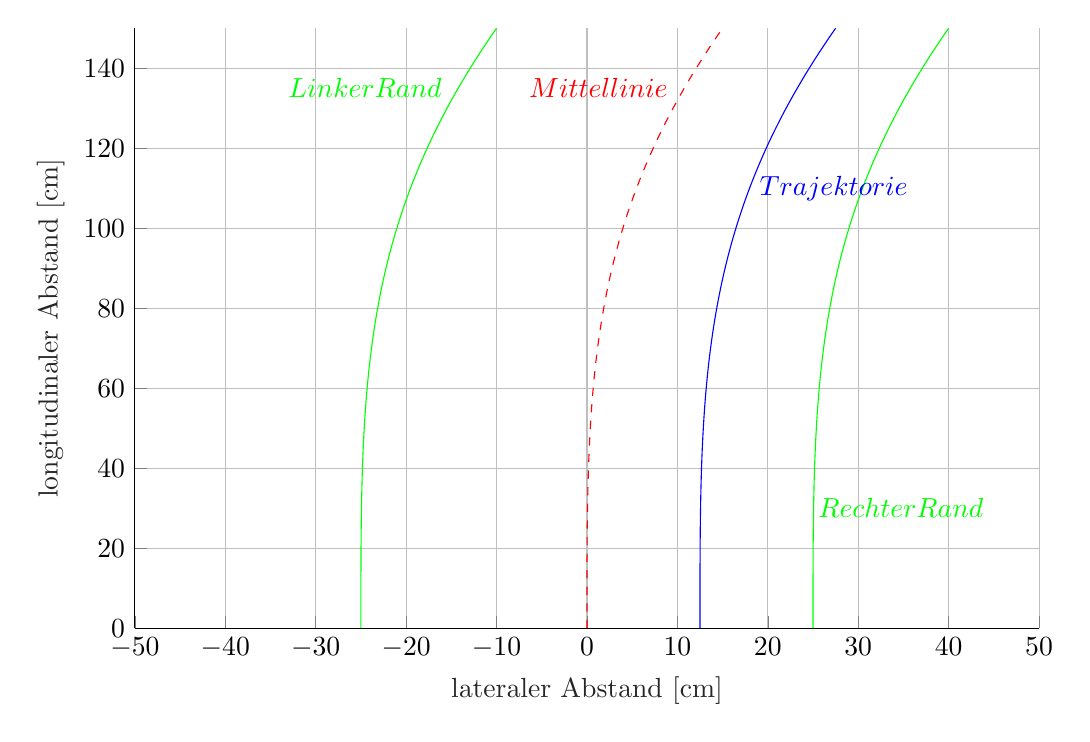
\begin{tikzpicture}

\begin{axis}[%
width=4.521in,
height=3.0in,
at={(0.758in,0.481in)},
scale only axis,
xmin=-50,
xmax=50,
xlabel style={font=\color{white!15!black}},
xlabel={lateraler Abstand [cm]},
ymin = 0,
ymax=150,
ylabel style={font=\color{white!15!black}},
ylabel={longitudinaler Abstand [cm]},
axis background/.style={fill=white},
axis x line*=bottom,
axis y line*=left
,
xmajorgrids,
ymajorgrids,
]

\draw[color=green] (-25,0) to[out=90,in=305-70] (-10,150);
\draw[color=green] (25,0) to[out=90,in=305-70] (40,150);
\draw[red, dashed] (0,0) to[out=90,in=305-70] (15,150);
\draw[color=blue] (12.5,0) to[out=90,in=305-70] (27.5,150);
\draw[color=green] (-15,135) node[left] {$Linker Rand$};
\draw[color=red] (10,135) node[left] {$Mittellinie$};
\draw[color=green] (24.5,30) node[right] {$Rechter Rand$};
\draw[color=blue] (18,110) node[right] {$Trajektorie$};



\end{axis}
\end{tikzpicture}%
%\end{document}
